\subsection{Validazione e Collaudo}
Questa fase comincia subito dopo la fase precedente e finisce con la data di consegna per la \textit{Revisione di Accettazione}, ovvero dal 09/04/2020 al 03/05/2020.\\
In questo periodo verranno creati ulteriori test per verificare il corretto funzionamento del prodotto. Se tutte le scadenze imposte dal gruppo vengono rispettate il tempo in eccesso viene occupato per la realizzazione di vincoli opzionali, concordati con il committente. 

\begin{itemize}
\item \textbf{Incremento e verifica dei documenti:} se fosse necessario, i documenti prodotti dal team verranno integrati.

 \item \textbf{Incremento e verifica delle attività}: sia la \textit{Technology baseline} che la \textit{Product Baseline} vengono eventualmente raffinate; particolare attenzione va alla codifica, svolta ad incrementi ciclici.

 \item \textbf{Verifica e collaudo}: vengono creati e applicati un set di test, che hanno lo scopo di portare il prodotto ad un buon livello qualitativo. Il gruppo si focalizzerà sulla sua correttezza e nel rispetto di tutti i requisiti.
\end{itemize}

\subsubsection{Periodi}
La pianificazione di questa fase è stata organizzata con le seguenti milestone:

\begin{itemize}
\item \textbf{09/04/2020 - 21/04/2020}: se fosse necessario, in questo periodo viene controllata tutta la documentazione e ci si dedicherà ad eventuali incrementi della \textit{Technology Baseline} e \textit{Product Baseline}.

\item \textbf{22/04/2020 - 01/05/2020}: entro la milestone del 01/05/2020 il gruppo ha come obbiettivo quello di completare la codifica del prodotto e dedicarsi al suo collaudo; se queste attività lo prevedono, verranno aggiornati nuovamente i documenti interessati.

\end{itemize}
\subsubsection{Diagramma di Gantt: Validazione e Collaudo}
\begin{figure}[h]
	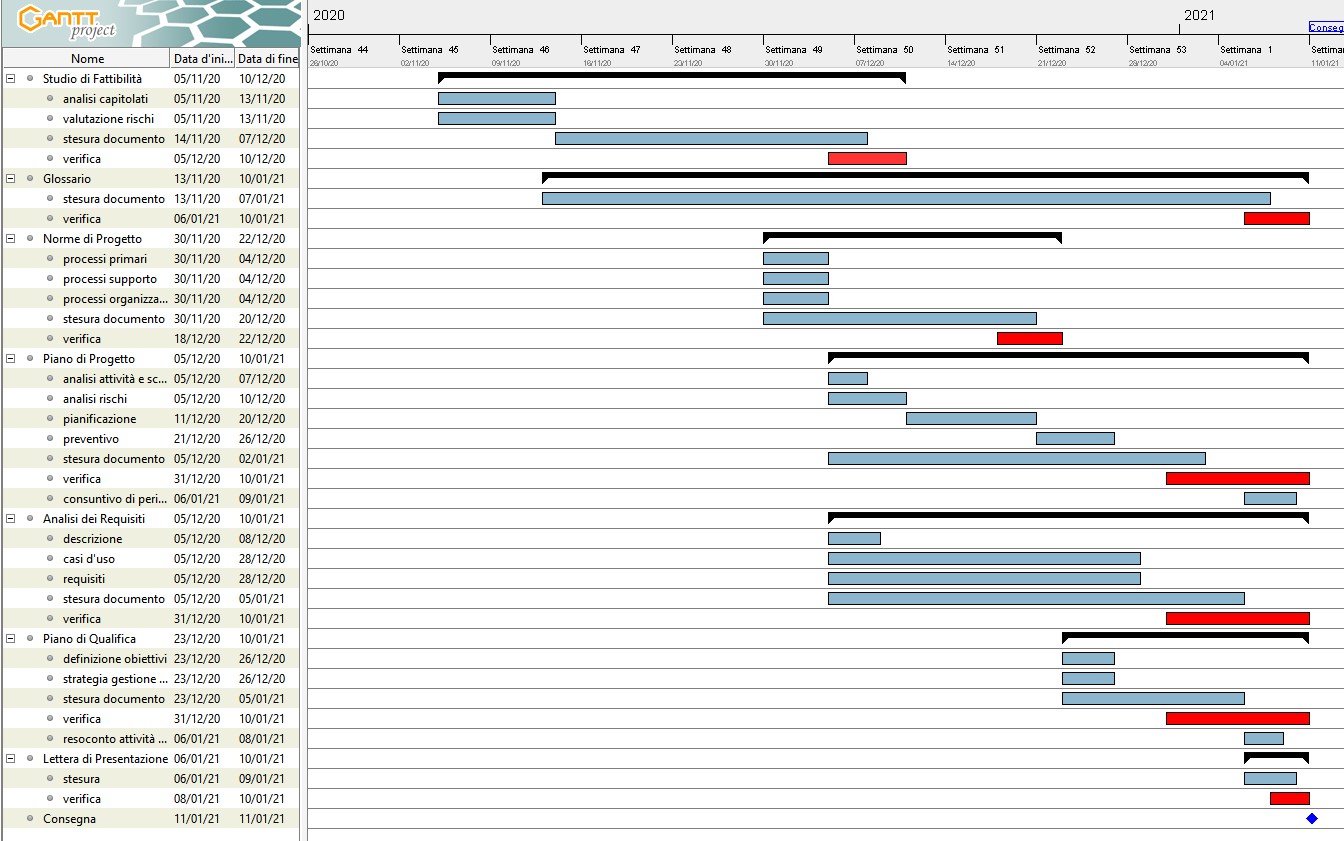
\includegraphics[scale=0.45]{Images/GanttPianificazioneAnalisi.PNG}
	\caption{Diagramma di Gantt dell'attività di Validazione e Collaudo}
\end{figure}